\section{Αρχιτεκτονική υλοποίησης} \label{section:4-3-implementation-architecture}

Το περιβάλλον ανάπτυξης της εφαρμογής υλοποιήθηκε χρησιμοποιώντας το μοντέλο αρχιτεκτονικής των μικροϋπηρεσιών. Το μοντέλο των μικροϋπηρεσιών βασίζεται στην αποδόμηση του συστήματος σε μικρές μονάδες, οι οποίες συνεργάζονται ώστε να προσφέρουν ένα ενιαίο αποτέλεσμα. Η προσέγγιση αυτή έχει πολλά πλεονεκτήματα σε σύγκριση με την ανάπτυξη μονολιθικών εφαρμογών. % todo: add reference
Ο βασικός λόγος για τον οποίο επιλέχθηκε η αρχιτεκτονική μικροϋπηρεσιών είναι η ευκολία που προσφέρει στη γρήγορη ανάπτυξη καινούργιων χαρακτηριστικών, ταυτόχρονα από διαφορετικά μέλη μίας ομάδας, ασύγχρονα και χωρίς την ανάγκη συνεχούς επικοινωνίας και συνεννόησης μεταξύ τους. Αυτό συμβαίνει επειδή κάθε μέρος του συστήματος (υπηρεσία) είναι αυτόνομο και η ανάπτυξή του είναι διαχωρισμένη από το υπόλοιπο σύστημα, με το οποίο είναι αδύναμα συνδεδεμένο (loosely coupled).

Το σύστημα του περιβάλλοντος ανάπτυξης συντίθεται από διάφορες μικροϋπηρεσίες, κάποιες από τις οποίες αναπτύχθηκαν στα πλαίσια αυτής της εργασίας, ενώ άλλες αποτελούν δωρεάν λογισμικό ανοιχτού κώδικα. Οι μικροϋπηρεσίες αυτές συνοψίζονται στον παρακάτω πίνακα:

\begin{table}[H]
    \begin{center}
        \begin{tabularx}{\textwidth}{l X}
            \toprule
            \textbf{Μικροϋπηρεσία} & \textbf{Σύντομη περιγραφή - Αντικείμενο/Στόχος} \\
            \midrule
            Concordia Application        & Υπηρεσία με την οποία αλληλεπιδρούν οι χρήστες \\ [0.5ex]
            Concordia Contracts Migrator & Υπηρεσία μεταφόρτωσης των συμβολαίων (contracts) στο blockchain \\ [0.5ex]
            Concordia Pinner             & Υπηρεσία καρφιτσώματος δεδομένων \\ [0.5ex]
            Concordia Contracts Provider & Υπηρεσία διαμοιρασμού των contract artifact μέσω HTTP \\ [0.5ex]
            Ganache                      & Τοπικό, ιδιωτικό Ethereum blockchain \\ [0.5ex]
            Rendezvous Server            & Υπηρεσία εύρεσης ομότιμων χρηστών \\ [0.5ex]
            \bottomrule
        \end{tabularx}
    \end{center}
    \caption{Σύντομη περιγραφή των υπηρεσιών του περιβάλλοντος ανάπτυξης}
    \label{table:4-3-microservice-summary}
\end{table}

Στα πλαίσια της εργασίας αναπτύχθηκαν επίσης διάφορα αρθρώματα (modules), κυρίως με τη μορφή βιβλιοθηκών JavaScript. Τα αρθρώματα χρησιμοποιούνται από τις υπηρεσίες για την επίτευξη των επιμέρους εργασιών. Η ανάπτυξη του λογισμικού σε ξεχωριστά αρθρώματα επιτρέπει την εύκολη επαναχρησιμοποίηση του κώδικα, καθώς και τον διαχωρισμό των αυτόνομων τμημάτων κώδικα. Τα αρθρώματα συνοψίζονται στον παρακάτω πίνακα:

\begin{table}[H]
    \begin{center}
        \begin{tabularx}{\textwidth}{l X}
            \toprule
            \textbf{Άρθρωμα} & \textbf{Σύντομη περιγραφή - Αντικείμενο/Στόχος} \\
            \midrule
            Άρθρωμα concordia-shared      & Χρήσιμα εργαλεία και σταθερές συστήματος \\ [0.5ex]
            Άρθρωμα concordia-contracts   & Μεταγλώττιση των contract και διάθεση των artifact \\ [0.5ex]
            Άρθρωμα eth-identity-provider & Δημιουργία μοναδικού αναγνωριστικού χρήστη για τη βάση OrbitDB \\ [0.5ex]
            Άρθρωμα drizzle               & Βελτιωμένη προγραμματιστική διεπαφή επικοινωνίας με το blockchain \\ [0.5ex]
            Άρθρωμα breeze                & Βελτιωμένη προγραμματιστική διεπαφή χρήσης της βάσης OrbitDB \\ [0.5ex]
            \bottomrule
        \end{tabularx}
    \end{center}
    \caption{Σύντομη περιγραφή των αρθρωμάτων του συστήματος}
    \label{table:4-3-software-units-summary}
\end{table}

\newpage
Τα αρθρώματα και οι υπηρεσίες περιγράφονται αναλυτικότερα σε επόμενες υποενότητες. Στο παρακάτω σχήμα φαίνεται η συνολική αρχιτεκτονική του συστήματος:

\vspace{\baselineskip}

\begin{figure}[H]
    \centering
    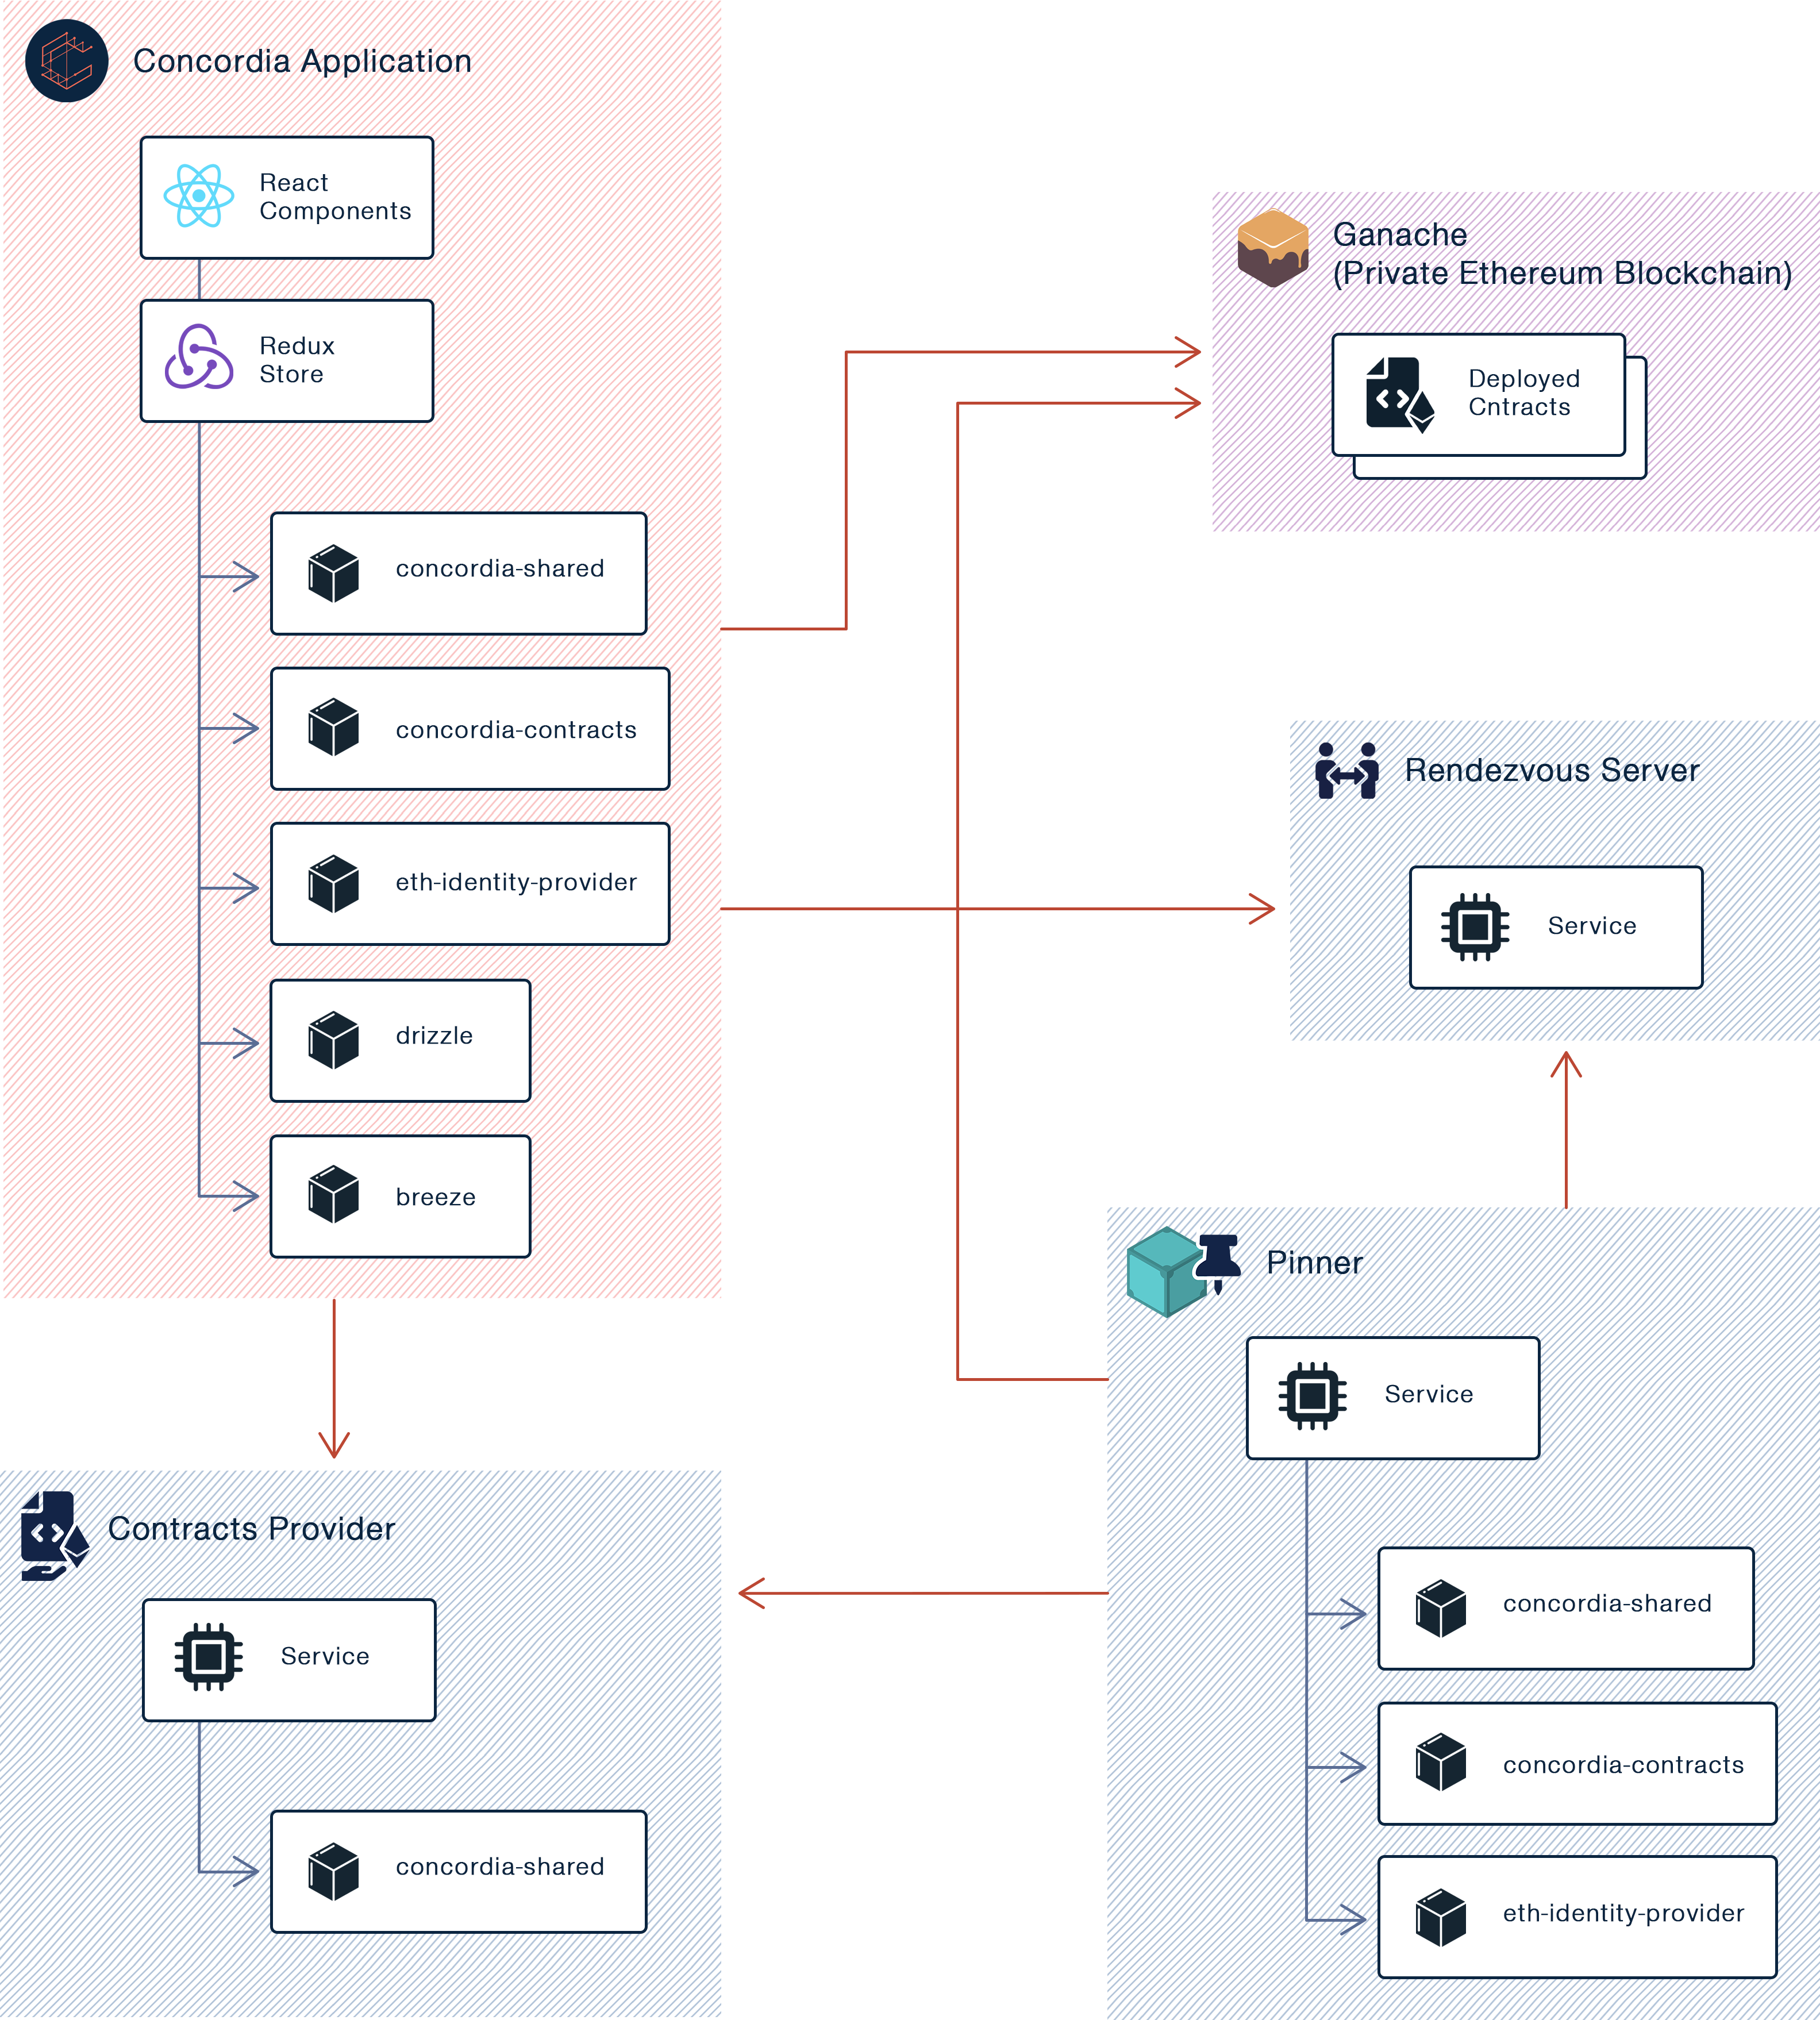
\includegraphics[width=\textwidth]{assets/figures/chapter-4/4.3.architecture-architecture-overview.png}
    \caption{Διάγραμμα αρχιτεκτονικής συστήματος}
    \label{figure:4-3-architecture-overview}
\end{figure}

\newpage
\subsection{Αρθρώματα} \label{subsection:4-3-1-software-units}

Σε αυτήν την υποενότητα θα περιγραφούν με μεγαλύτερη λεπτομέρεια τα αρθρώματα που αναπτύχθηκαν.

\subsubsection{Άρθρωμα concordia-shared} \label{subsubsection:4-3-1-concordia-shared-unit}

Το άρθρωμα concordia-shared αποτελεί μία βιβλιοθήκη χρήσιμων εργαλείων και σταθερών. Εδώ περιέχεται όλο το λογισμικό το οποίο πρέπει ή είναι επιθυμητό να συμπεριφέρεται με τον ίδιο τρόπο συνολικά στο σύστημα, όπως για παράδειγμα μέθοδοι παραμετροποίησης των υπηρεσιών και μέθοδοι καταγραφής (logging). Το άρθρωμα αυτό χρησιμοποιείται από το άρθρωμα \hyperref[subsubsection:4-3-1-concordia-contracts-unit]{concordia-contracts} καθώς και από τις υπηρεσίες \hyperref[subsection:4-3-2-concordia-application-service]{Concordia Application}, \hyperref[subsection:4-3-4-concordia-pinner-service]{Concordia Pinner} και \hyperref[subsection:4-3-5-concordia-contracts-provider-service]{Concordia Contracts Provider}.

Το άρθρωμα αυτό γίνεται διαθέσιμο για χρήση με τη μορφή τοπικής βιβλιοθήκης με τη χρήση της δυνατότητας διαχείρισης μοναδικού αποθετηρίου κώδικα (monorepo) yarn workspaces{\footnote{\url{https://yarnpkg.com/features/workspaces}}}.
\subsubsection{Άρθρωμα concordia-contracts} \label{subsubsection:4-3-1-concordia-contracts-unit}

Το άρθρωμα αυτό επιτελεί δύο ενέργειες. Αρχικά, είναι το άρθρωμα στο οποίο αναπτύσσονται τα contracts που χρησιμοποιούνται από την εφαρμογή. Το άρθρωμα αυτό αναλαμβάνει τη μεταγλώττιση των contracts από κώδικα γλώσσας Solidity, στην κατάλληλη τελική μορφή JSON. Παρέχονται επίσης σενάρια ενεργειών (scripts) ώστε τα contracts να μεταφορτωθούν σε blockchain καθώς και στην υπηρεσία \hyperref[subsection:4-3-5-concordia-contracts-provider-service]{Concordia Contracts Provider}. Αποτελεί επίσης βιβλιοθήκη η οποία μετά τη μεταγλώττιση και μεταφόρτωση των contracts σε blockchain παρέχει τα contract artifacts. Χρησιμοποιείται από τις υπηρεσίες \hyperref[subsection:4-3-2-concordia-application-service]{Concordia Application} και \hyperref[subsection:4-3-4-concordia-pinner-service]{Concordia Pinner}.

Το άρθρωμα αυτό γίνεται διαθέσιμο για χρήση με τη μορφή τοπικής βιβλιοθήκης με τη χρήση της δυνατότητας yarn workspaces.
\subsubsection{Άρθρωμα eth-identity-provider} \label{subsubsection:4-3-1-eth-identity-provider-unit}

Η λειτουργία της βάσης OrbitDB επιτρέπει τη χρήση προσαρμοσμένων  orbit-db-identity-provider, οι οποίοι θα δημιουργούν και θα επικυρώνουν
τα μοναδικά αναγνωριστικά των χρήστών (OrbitDB Identity) βάσει προσαρμοσμένων εξωτερικών αναγνωριστικών (external identifier), όπως παρουσιάζεται στο σχήμα \ref{figure:4-2-4-2-orbit-db-identity}. 

Στην περίπτωση της εφαρμογής Concordia είναι χρήσιμο να μπορούν να υπολογιστούν με ντετερμινιστικό τρόπο οι OrbitDB βάσεις δεδομένων του κάθε χρήστη, για λόγους απλότητας και εξοικονόμησης αποθηκευτικού χώρου επί του blockchain. Έτσι, αφού κάθε χρήστης ορίζεται μοναδικά μέσω της διεύθυνσης Ethereum με την οποία εγγράφεται και συνδέεται, αυτή θα πρέπει να αποτελεί και το εξωτερικό αναγνωριστικό στο πεδίο id της OrbitDB Identity.

Για αυτόν το λόγο υλοποιήθηκε το άρθρωμα eth-identity-provider, το οποίο:

\begin{itemize}
	\item Παράγει ένα OrbitDB Identity για τον χρήστη, με id τον συνδυασμο του Ethereum address του και του address του κεντρικού contract της εφαρμογής\footnote{Το δεύτερο εισήχθη για την αποφυγή προβλημάτων σε πολλαπλές αναπτύξεις συμβολαίων.}. Αυτό επιτυγχάνεται με την υπογραφή μίας συναλλαγής με το Ethereum private key του χρήστη, μέσω του MetaMask.
	\item Επικυρώνει τις OrbitDB Identity που απαιτούνται, εξασφαλίζοντας ότι υπογράφηκαν από τα Ethereum private key των κατόχων τους. 
	\item Διασφαλίζει ντετερμινιστικές, υπολογίσιμες διευθύνσεις OrbitDB βάσεων για τον κάθε χρήστη.
\end{itemize}

Αυτό το άρθρωμα γίνεται διαθέσιμο για χρήση με τη μορφή βιβλιοθήκης μέσω του μητρώου λογισμικού npm (\url{https://www.npmjs.com/package/@ecentrics/eth-identity-provider}), ενώ το αποθετήριό του βρίσκεται στο GitLab (\url{https://gitlab.com/ecentrics/eth-identity-provider}).

\subsubsection{Άρθρωμα drizzle} \label{subsubsection:4-3-1-drizzle-unit}

Το άρθρωμα drizzle που χρησιμοποιείται στην υπηρεσία \hyperref[subsection:4-3-2-concordia-application-service]{Concordia Application} είναι μία τροποποιημένη έκδοση της JavaScript βιβλιοθήκης Drizzle (και συγκεκριμένα του @drizzle/store\footnote{\url{https://github.com/trufflesuite/drizzle/tree/develop/packages/store}}), η οποία προσφέρεται από τη σουίτα εργαλείων Truffle. Η τροποποιημένη βιβλιοθήκη αναπτύχθηκε στα πλαίσια της διπλωματικής με στόχο τη διευκόλυνση της χρήσης του Drizle και την επιδιόρθωση προβληματικών σημείων της πρωτότυπης βιβλιοθήκης.

Το άρθρωμα drizzle υλοποιεί τις προγραμματιστικές διεπαφές μέσω των οποίων πραγματοποιείται η επικοινωνία της εφαρμογής με το blockchain. Για την επίτευξη της επικοινωνίας αυτής, η βιβλιοθήκη χρησιμοποιεί τη συλλογή βιβλιοθηκών web3.js η οποία αποτελεί τον πιο διαδεδομένο τρόπο διεπαφής με το blockchain σε αποκεντρωτικές εφαρμογές. Τελικά, παρέχει ένα \hyperref[subsection:4-2-2-2-redux]{Redux} store, το οποίο συμπεριλαμβάνεται στο κεντρικό store της εφαρμογής.

Το άρθρωμα αυτό γίνεται διαθέσιμο για χρήση με τη μορφή βιβλιοθήκης μέσω του μητρώου λογισμικού npm\footnote{\url{https://www.npmjs.com/package/@ecentrics/drizzle}}, ενώ το αποθετήριό του βρίσκεται στο GitLab\footnote{\url{https://gitlab.com/ecentrics/drizzle}}.
\subsubsection{Άρθρωμα breeze} \label{subsubsection:4-3-1-breeze-unit}

Το άρθρωμα αυτό αναπτύχθηκε στα πλαίσια της διπλωματικής εργασίας και αποτελεί μία βιβλιοθήκη περίβλημα (wrapper) της βιβλιοθήκης OrbitDB, η οποία παρέχει ένα Redux store. 

Με τη συμπερίληψη του store του αρθρώματος στο κεντρικό Redux store της εφαρμογής, παρέχεται η δυνατότητα εκτέλεσης των λειτουργιών των OrbitDB βάσεων εντός του γενικότερου flow του frontend της εφαρμογής. Έτσι, οι προγραμματιστικές διεπαφές που προσφέρει η Orbit χρησιμοποιούνται πλέον μέσα από actions, reducers και middleware.

Το άρθρωμα αυτό γίνεται διαθέσιμο για χρήση με τη μορφή βιβλιοθήκης μέσω του μητρώου λογισμικού npm \footnote{\url{https://www.npmjs.com/package/@ecentrics/breeze}}, ενώ το αποθετήριό του βρίσκεται στο GitLab \footnote{\url{https://gitlab.com/ecentrics/breeze}}.

\subsection{Concordia Application} \label{subsection:4-3-2-concordia-application-service}

\subsubsection{Περιγραφή - Στόχοι υπηρεσίας}

\logo{chapter-4/4.3.concordia-logo}{Concordia logo}

Η εφαρμογή Concordia (Concordia Application) εκθέτει τις γραφικές διεπαφές μέσω των οποίων αλληλεπιδρούν οι χρήστες με το σύστημα. Αποτελεί τον δίαυλο επικοινωνίας του τελικού χρήστη με το blockchain και με τη βάση OrbitDB. Η αρχιτεκτονική της υπηρεσίας φαίνεται στο σχήμα \ref{figure:4-3-concordia-application-architecture}.

Μέσω της εφαρμογής Concordia οι χρήστες μπορούν:

\begin{itemize}
    \item Να περιηγούνται και να διαβάζουν το περιεχόμενο της πλατφόρμας

    \item Να δημιουργήσουν λογαριασμό χρήστη

    \item Να δημοσιεύουν και να τροποποιούν προσωπικές τους πληροφορίες, όπως την τοποθεσία και την εικόνα προφίλ

    \item Να δημιουργούν θέματα (topics)

    \item Να δημιουργούν και να τροποποιούν μηνύματα (posts)

    \item Να δημιουργούν ψηφοφορίες (polls), καθώς και να ψηφίζουν σε αυτές (εφόσον έχουν το δικαίωμα)

    \item Να υπερψηφίζουν (up-vote) ή να καταψηφίζουν (down-vote) μηνύματα άλλων χρηστών
\end{itemize}

Η υπηρεσία αποτελείται από κώδικα γραμμένο σε JavaScript, ο οποίος γίνεται διαθέσιμος στους τελικούς χρήστες με τη μορφή εφαρμογής διαδικτύου (web application) μέσω ενός διακομιστή (server). Παρόλο που η υπηρεσία προσφέρει τη γραφική διεπαφή χρήστη μόνο στην αγγλική γλώσσα, έχει παραμετροποιηθεί ώστε να είναι δυνατή η εύκολη μεταγλώττισή της χωρίς την ανάγκη πραγματοποίησης μεγάλων αλλαγών στον κώδικα.

Χρησιμοποιείται η βιβλιοθήκη \hyperref[subsection:4-2-2-1-react]{React} για την οργάνωση και την ανάπτυξη των συνθετικών τμημάτων (components) του γραφικού περιβάλλοντος. Για το γραφικό περιβάλλον γίνεται χρήση του framework της Semantic UI\footnote{\url{https://semantic-ui.com/}}. Χρησιμοποιείται η βιβλιοθήκη \hyperref[subsection:4-2-2-2-redux]{Redux} για τη διαχείριση κατάστασης της εφαρμογής (state management),
καθώς και η βιβλιοθήκη \hyperref[subsection:4-2-2-3-redux-saga]{Redux-Saga} για τη διαχείριση ασύγχρονων παράπλευρων ενεργειών (side-effects) σε ένα σύστημα βασισμένο σε συμβάντα (event-based). Άλλες βιβλιοθήκες χρησιμοποιούνται για διάφορα μέρη της υπηρεσίας, ενώ χρησιμοποιούνται επίσης τα αρθρώματα που περιγράφηκαν προηγουμένως για την επίτευξη διαφορετικών στόχων. Ο πλήρης κατάλογος των βιβλιοθηκών και αρθρωμάτων μπορεί να βρεθεί στον κώδικα της υπηρεσίας\footnote{\url{https://gitlab.com/ecentrics/concordia/-/blob/master/packages/concordia-app/package.json}}.

\vspace{\baselineskip}

\begin{figure}[H]
    \centering
    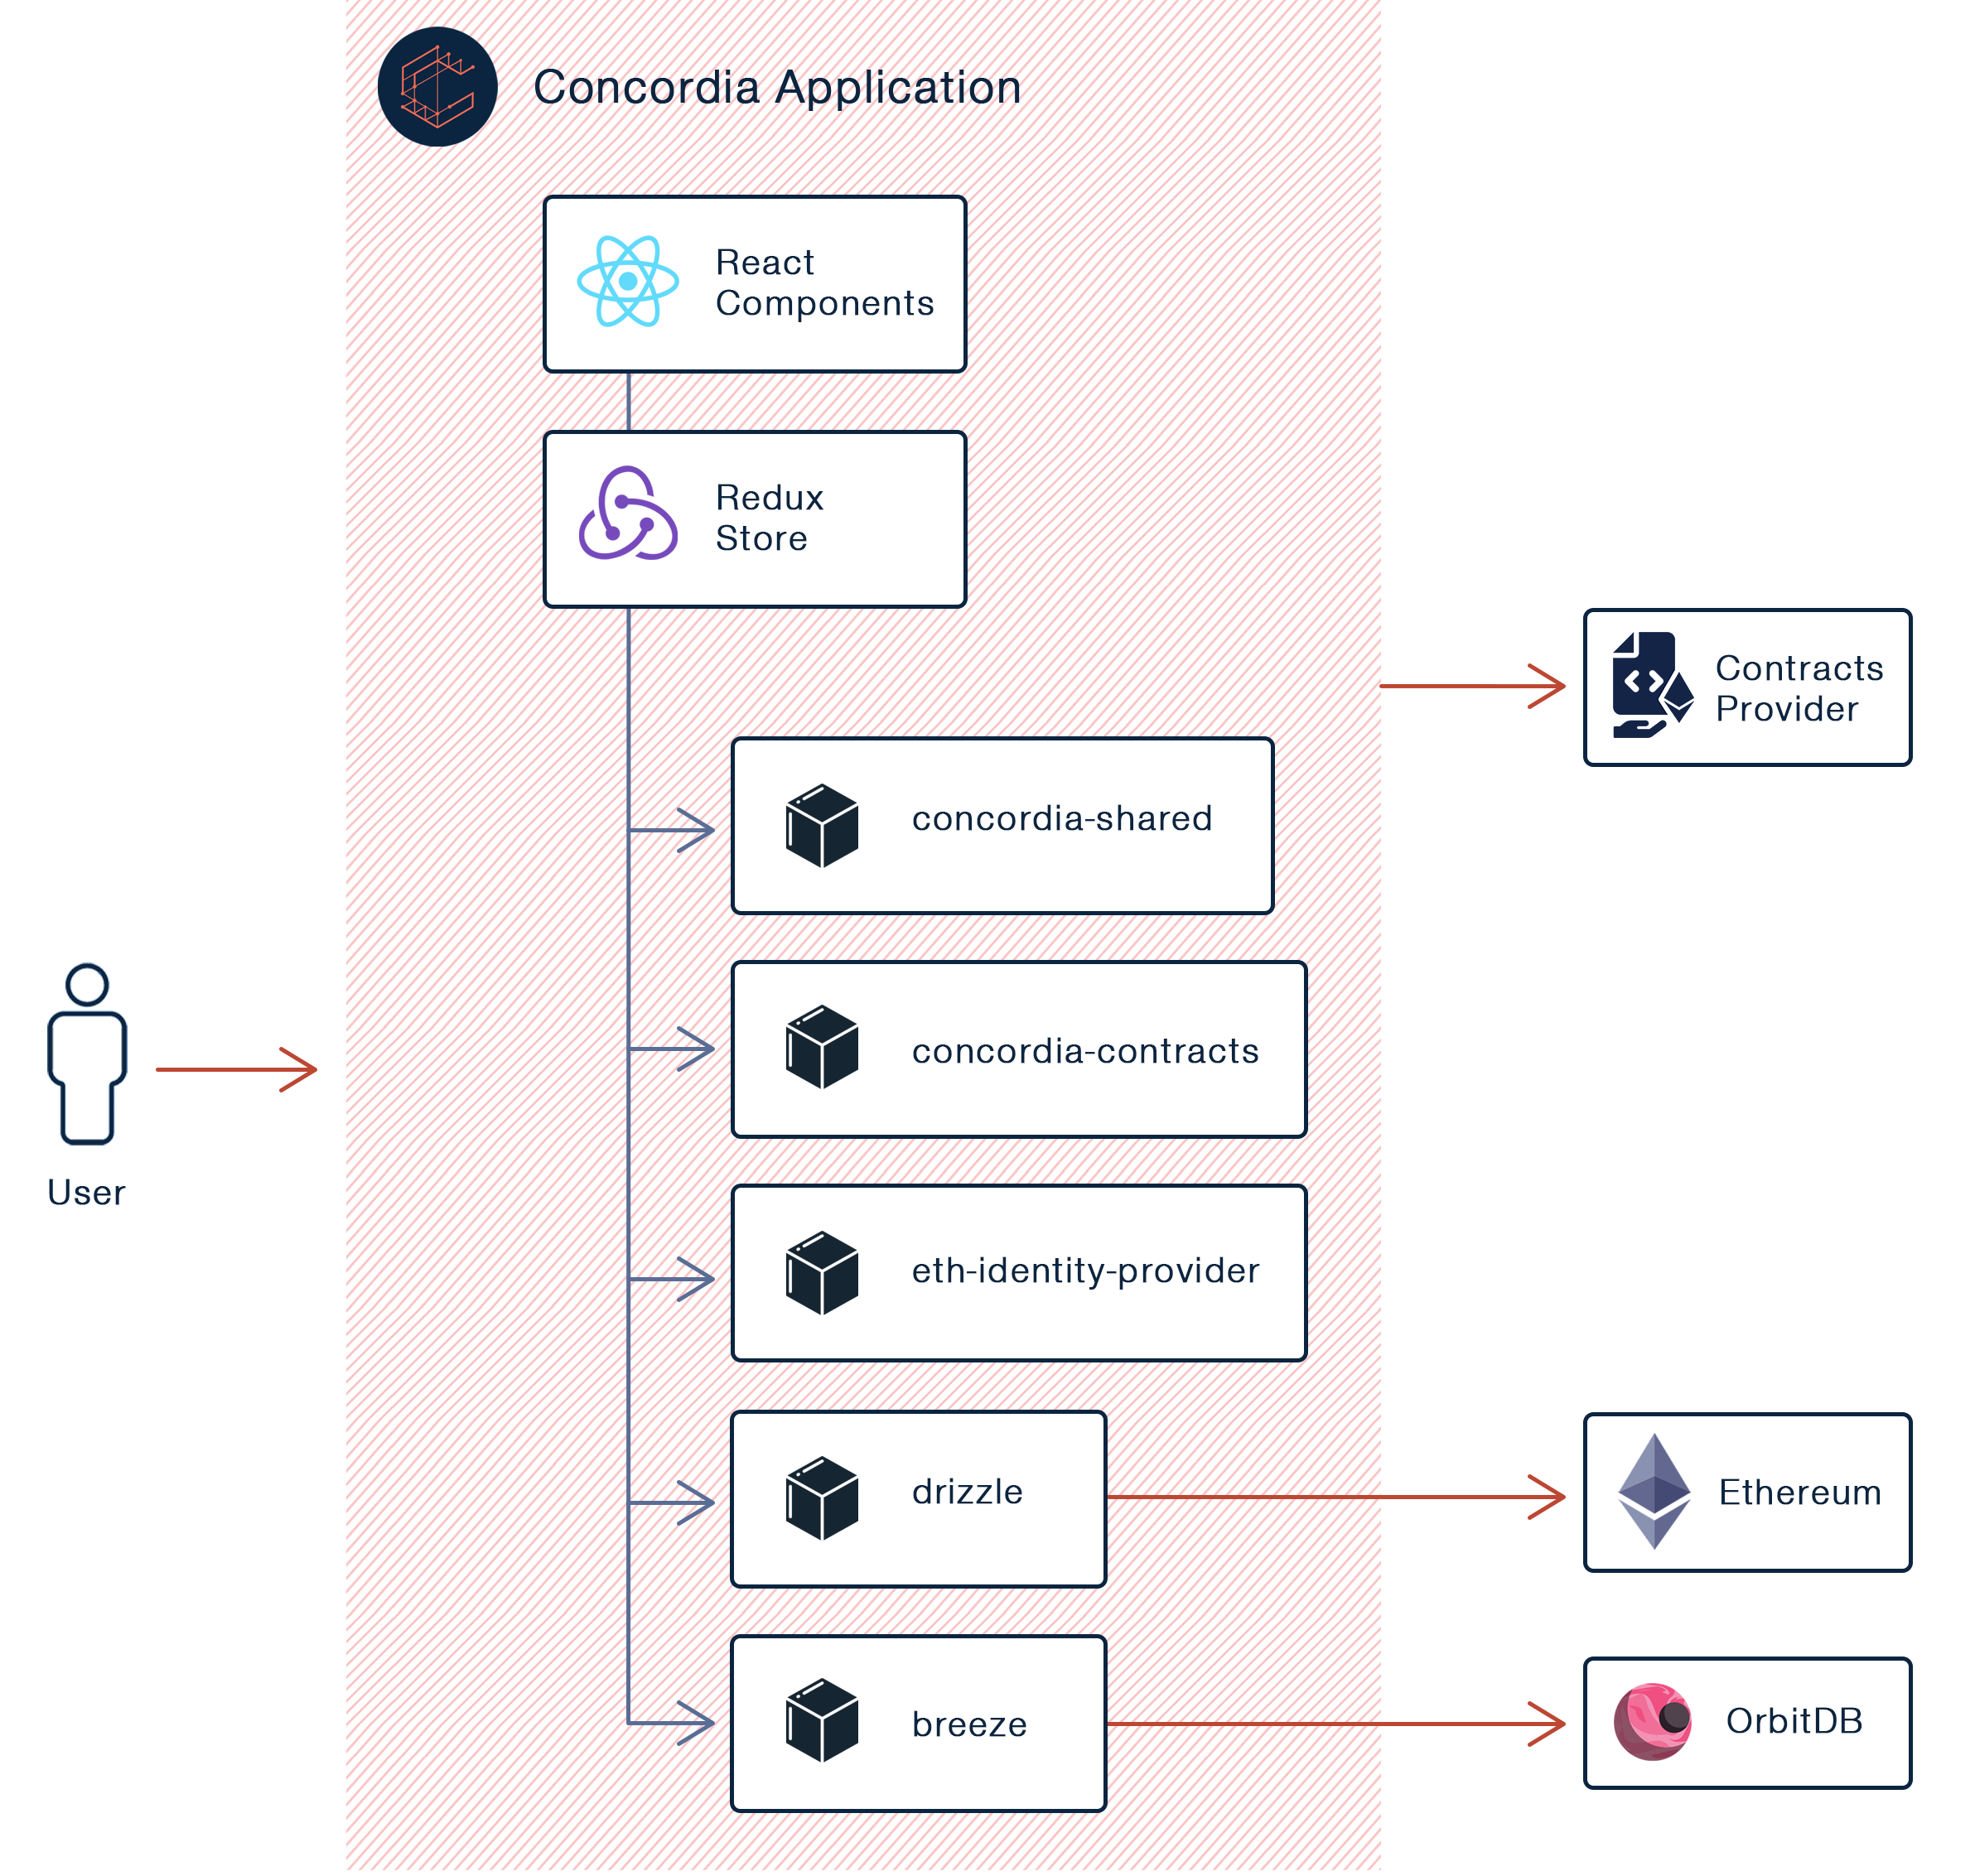
\includegraphics[width=.9\textwidth]{assets/figures/chapter-4/4.3.architecture-4.3.2.concordia-application-architecture.png}
    \caption{Αρχιτεκτονική υπηρεσίας Concordia Application}
    \label{figure:4-3-concordia-application-architecture}
\end{figure}

Για τη λειτουργία της υπηρεσία Concordia Application είναι απαραίτητα τα αντικείμενα (artifacts) που προκύπτουν από τη μεταγλώττιση των contract και τη μεταφόρτωση/ δημοσίευσή τους στο blockchain. Για την εισαγωγή των artifact στην υπηρεσία έχουν αναπτυχθεί δύο μέθοδοι.

Η πρώτη μέθοδος είναι η μεταγλώττιση και μεταφόρτωση των contract πριν την παραγωγή του πακέτου λογισμικού της υπηρεσίας για τελική χρήση (production build). Με αυτόν τον τρόπο η υπηρεσία θα έχει πρόσβαση στα artifact μέσω της βιβλιοθήκης που παράγεται από το άρθρωμα concordia-contracts. Αυτή η μέθοδος έχει το μειονέκτημα ότι το τελικό πακέτο λογισμικού (production build) "δένεται" με όποια συγκεκριμένη έκδοση των contract είναι διαθέσιμη κατά τη δημιουργία του πακέτου. Αυτό σημαίνει ότι σε ενδεχόμενη ενημέρωση των contract πρέπει αναγκαστικά να δημιουργηθεί και νέα έκδοση του πακέτου λογισμικού της υπηρεσίας Concordia Application.

Για την αποφυγή του παραπάνω προβλήματος αναπτύχθηκε η δεύτερη μέθοδος προσκόμισης των contract artifact, η οποία είναι η λήψη τους (download) από μία άλλη τοποθεσία στο διαδίκτυο. Σε αυτή τη μέθοδο, η εφαρμογή κατά την εκκίνησή της πραγματοποιεί ένα HTTP αίτημα (HTTP request) σε διεύθυνση η οποία δίνεται ως μεταβλητή περιβάλλοντος (environment variable). Η απάντηση του αιτήματος αναμένεται να περιέχει τα artifact ώστε η εφαρμογή να τα χρησιμοποιήσει.

\subsubsection{Διανομή}

Η υπηρεσία Concordia Application πακετάρεται μαζί με τον διακομιστή nginx και γίνεται διαθέσιμη για χρήση ως εικόνα Docker (Docker image) μέσω του αποθετηρίου εικόνων Docker Hub\footnote{\url{https://hub.docker.com/r/ecentrics/concordia-app}}. Κατά την εκτέλεση της εικόνας, οι χρήστες μπορούν, μέσω μεταβλητών περιβάλλοντος, να ορίσουν παραμέτρους της εκτέλεσης, όπως τη διεύθυνση του εξυπηρετητή (host location) της εφαρμογής και τις τοποθεσίες των υπηρεσιών Rendezvous Server και Contracts Provider.
\subsection{Concordia Contracts Migrator} \label{subsection:4-3-3-concordia-contracts-migrator}

\subsubsection{Περιγραφή - Στόχοι υπηρεσίας}

Η υπηρεσία αυτή αποτελείται από ένα εκτελέσιμο πρόγραμμα γραμμής εντολών βασισμένο στο άρθρωμα concordia-contracts που αναλύθηκε σε προηγούμενη υποενότητα (\ref{subsection:4-3-1-software-units}). Το πρόγραμμα, κατά την εκτέλεσή του, μεταγλωττίζει τα contract και έπειτα τα μεταφορτώνει στο blockchain το οποίο είναι ορισμένο με χρήση μεταβλητών περιβάλλοντος. Τέλος, αν οι κατάλληλες μεταβλητές περιβάλλοντος είναι ορισμένες, το πρόγραμμα μεταφορτώνει τα τελικά artifacts σε αποθετήριο Concordia Contracts Provider. Η αρχιτεκτονική της υπηρεσίας φαίνεται στο σχήμα \ref{figure:4-3-concordia-contracts-migrator-architecture}.

\vspace{.5\baselineskip}

\begin{figure}[H]
    \centering
    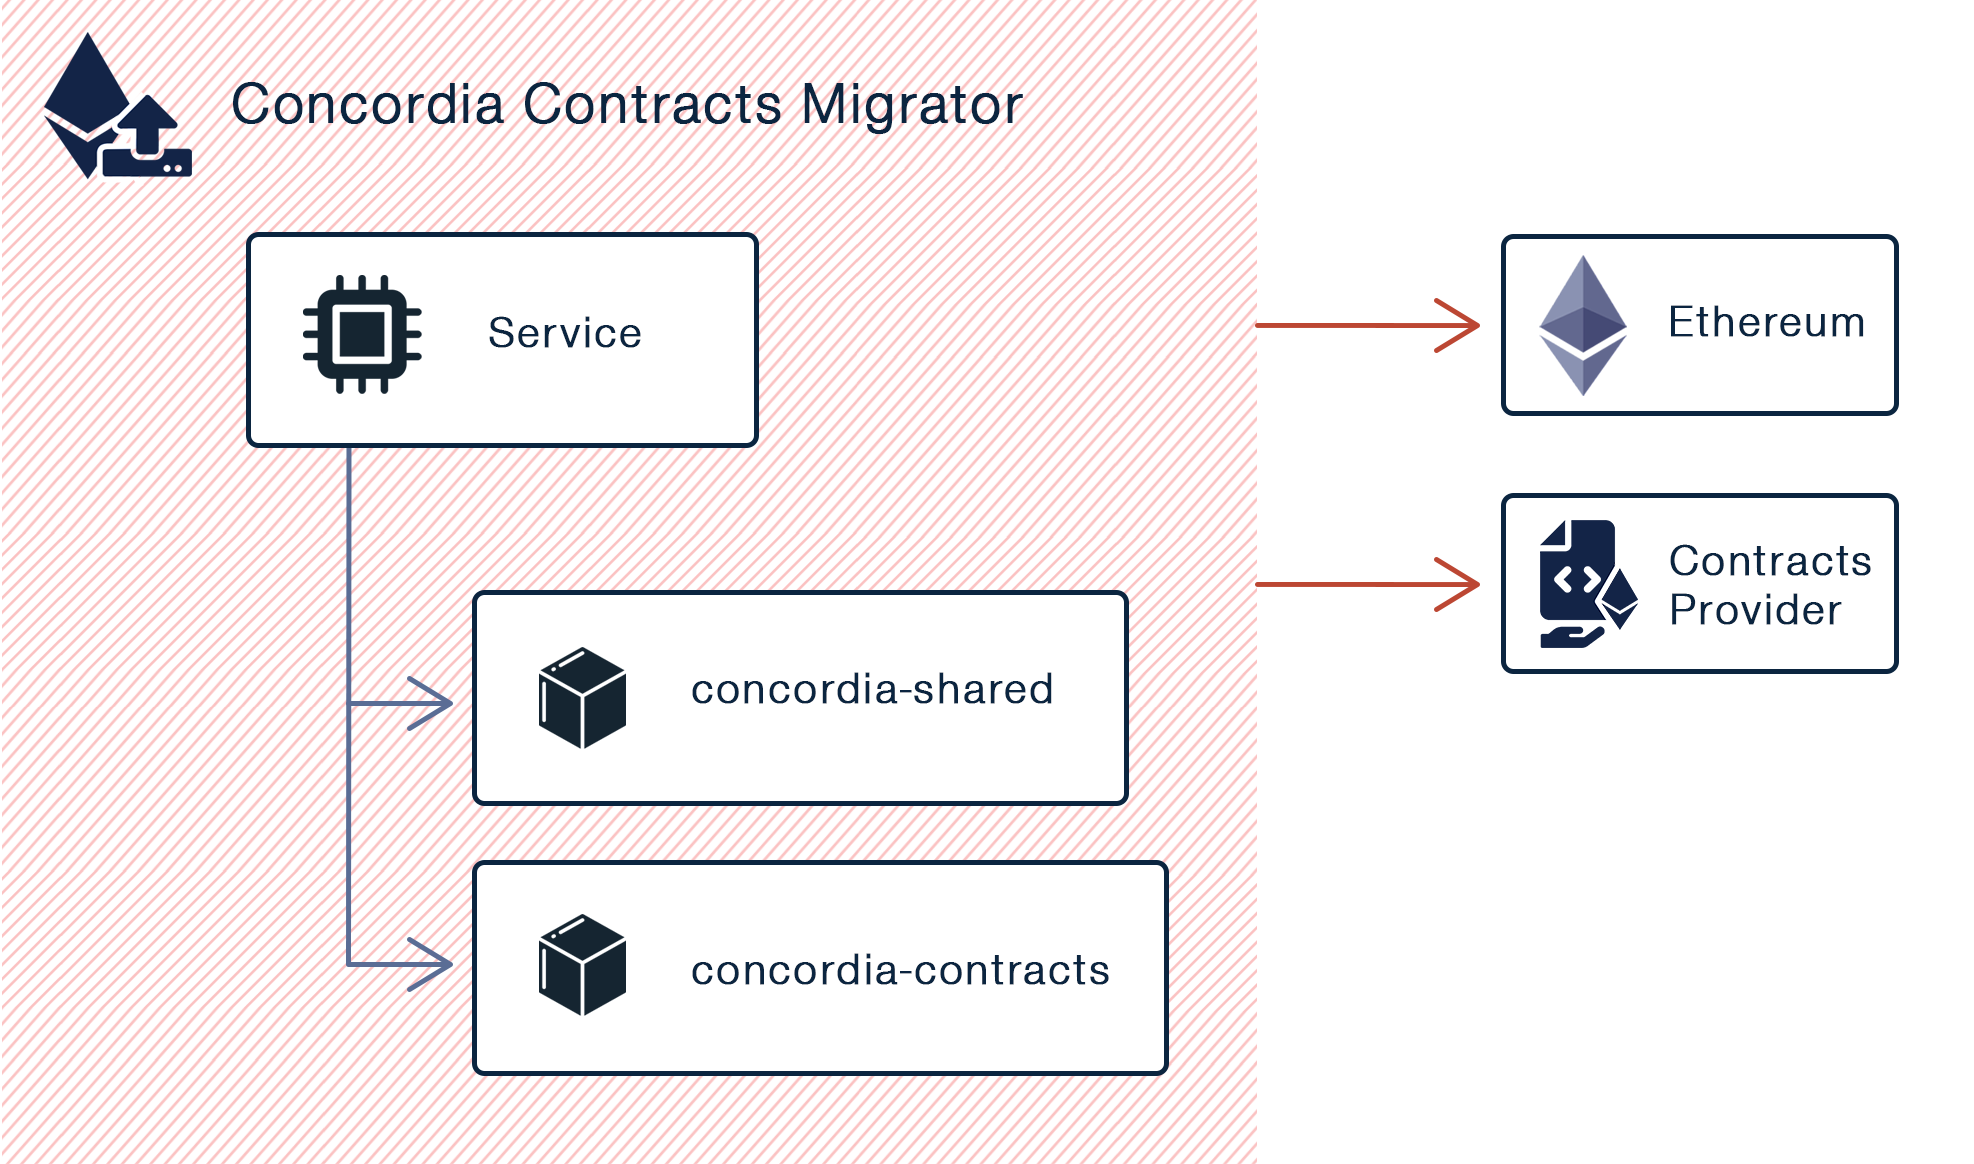
\includegraphics[width=.75\textwidth]{assets/figures/chapter-4/4.3.architecture-4.3.3.concordia-contracts-migrator-architecture.png}
    \caption{Αρχιτεκτονική υπηρεσίας Concordia Contracts Migrator}
    \label{figure:4-3-concordia-contracts-migrator-architecture}
\end{figure}

\subsubsection{Διανομή}

Η υπηρεσία αυτή γίνεται διαθέσιμη για χρήση ως Docker image μέσω του αποθετηρίου εικόνων Docker Hub. Οι χρήστες μπορούν χρησιμοποιώντας μεταβλητές περιβάλλοντος να αλλάξουν τη διεύθυνση του blockchain και την τοποθεσία της υπηρεσίας Contracts Provider στην οποία το πρόγραμμα θα μεταφορτώσει τα contract και τα artifact.
\subsection{Concordia Pinner} \label{subsection:4-3-4-concordia-pinner-service}

\subsubsection{Περιγραφή - Στόχοι υπηρεσίας}

Η υπηρεσία καρφιτσώματος περιεχομένου (Concordia Pinner) αποτελεί μία εφαρμογή τερματικού (temrinal application/cmd application) η οποία στοχεύει στο καρφίτσωμα (pinning) του περιεχομένου που αποθηκεύεται στο IPFS μέσω της βάσης OrbitDB. Η υπηρεσία είναι γραμμένη στη γλώσσα προγραμματισμού JavaScript. Η αρχιτεκτονική της υπηρεσίας φαίνεται το σχήμα \ref{figure:4-3-concordia-pinner-architecture}.

\begin{figure}[H]
    \centering
    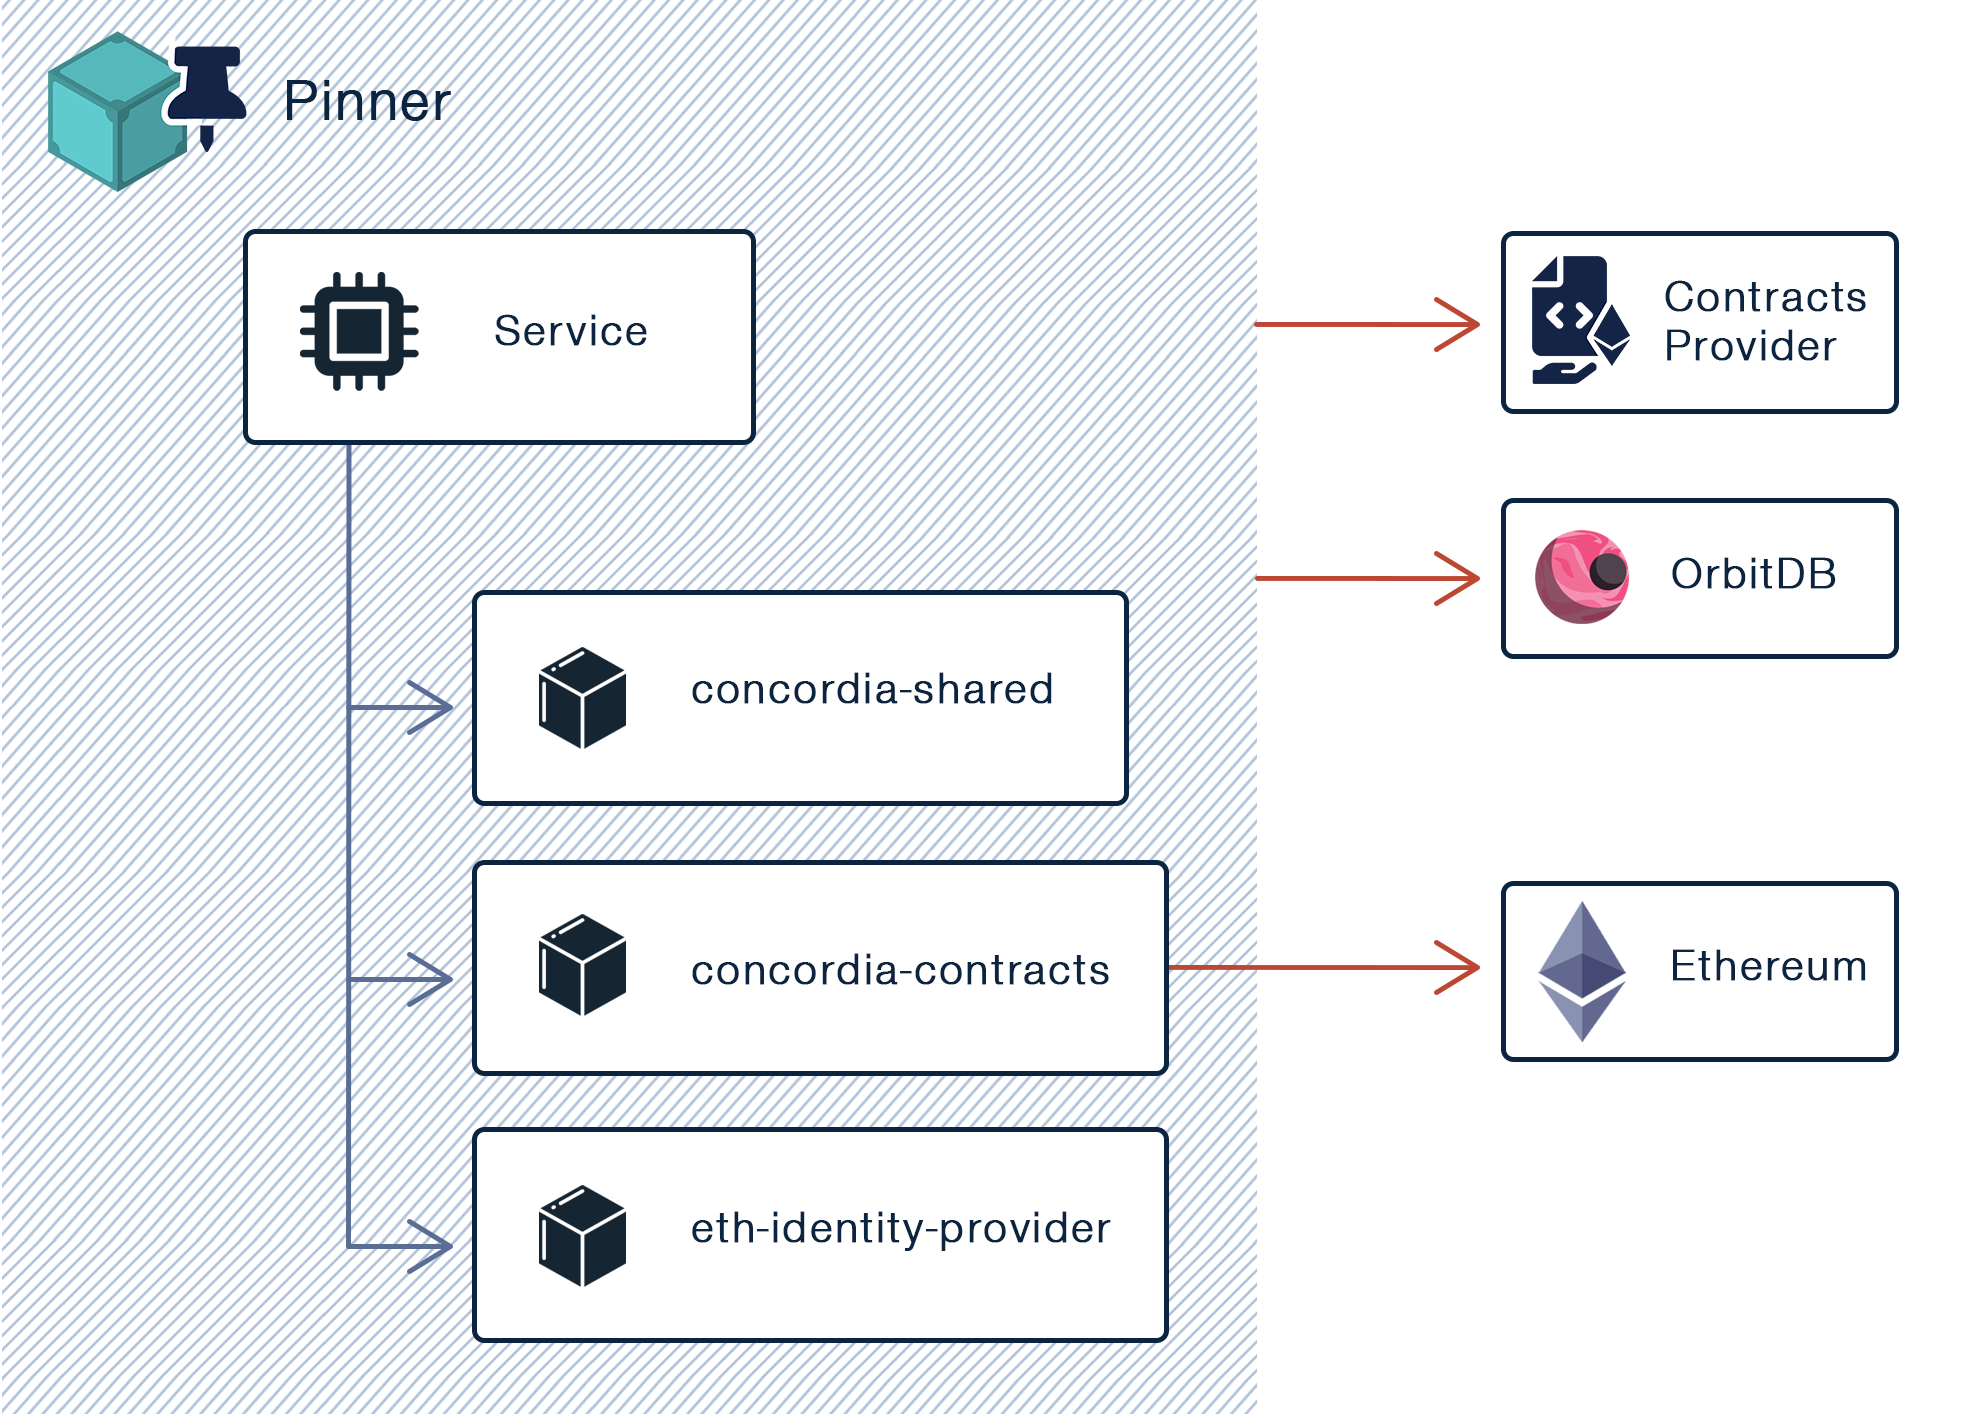
\includegraphics[width=.6\textwidth]{assets/figures/chapter-4/4.3.architecture-4.3.4.concordia-pinner-architecture.png}
    \caption{Αρχιτεκτονική υπηρεσίας Concordia Pinner}
    \label{figure:4-3-concordia-pinner-architecture}
\end{figure}

Η υπηρεσία αυτή υλοποιήθηκε για να εγγυηθεί η διαθεσιμότητα του περιεχομένου του συστήματος που αποθηκεύεται στο IPFS (τίτλοι θεμάτων, περιεχόμενο μηνυμάτων και άλλα). Λόγω του τρόπου λειτουργίας του IPFS, το περιεχόμενο που αναρτούν οι χρήστες πρέπει να καρφιτσώνεται από άλλους χρήστες ή αυτόνομες εφαρμογές, όπως η υπηρεσία Concordia Pinner, ώστε να είναι διαθέσιμο. Αν το περιεχόμενο δεν καρφιτσωθεί, τότε θα είναι διαθέσιμο στους υπόλοιπους χρήστες μόνο από
τον δημιουργό του, έτσι αν αυτός δεν είναι ενεργός στο δίκτυο, το περιεχόμενο θα είναι αδύνατο να βρεθεί.

Η υπηρεσία συνδέεται στο blockchain από όπου παρακολουθεί την κατάσταση του συστήματος και "ακούει" για νέους χρήστες, θέματα, μηνύματα και ψηφοφορίες. Η υπηρεσία συνδέεται επίσης στο IPFS, έτσι όταν δημιουργηθεί νέο περιεχόμενο στο σύστημα το καρφιτσώνει αυτόματα. Με αυτό τον τρόπο, διατηρώντας την υπηρεσία πάντα διαθέσιμη, για παράδειγμα εκτελώντας τη σε περιβάλλον διακομιστή (server), διαβεβαιώνεται η διαθεσιμότητα του περιεχομένου.

\subsubsection{Διανομή}

Η υπηρεσία αυτή γίνεται διαθέσιμη για χρήση ως docker image μέσω του αποθετηρίου εικόνων dockerhub. Κατά την εκτέλεση της εικόνας οι χρήστες μπορούν μέσω μεταβλητών περιβάλλοντος να ορίσουν παραμέτρους της υπηρεσίας όπως τη διεύθυνση του εξυπηρετητή (host location), τη διεύθυνση του blockchain, τις διαδρομές αποθήκευσης των δεδομένων στο σύστημα και τις τοποθεσίες των υπηρεσιών Rendezvous Server και Contracts Provider.
\subsection{Concordia Contracts Provider} \label{subsection:4-3-5-concordia-contracts-provider-service}

\subsubsection{Περιγραφή - Στόχοι υπηρεσίας}

Η υπηρεσία Contracts Provider αποτελεί μία βοηθητική υπηρεσία η οποία υλοποιεί ένα απλό αποθετήριο για τα \textenglish{contract artifact}. Είναι γραμμένη σε JavaScript και διαθέτει δύο HTTP \textenglish{endpoint}, ένα για τη μεταφόρτωση (upload) των artifact προς την υπηρεσία και ένα για τη λήψη (download) από την υπηρεσία. Η υπηρεσία υποστηρίζει επίσης την επισύναψη ετικετών στα artifact, όπως της έκδοσης (version) ή του κλαδιού ανάπτυξης (για παράδειγμα \textenglish{master/develop}). Η αρχιτεκτονική της φαίνεται στο σχήμα \ref{figure:4-3-concordia-contracts-provider-architecture}.

\vspace{.5\baselineskip}

\begin{figure}[H]
    \centering
    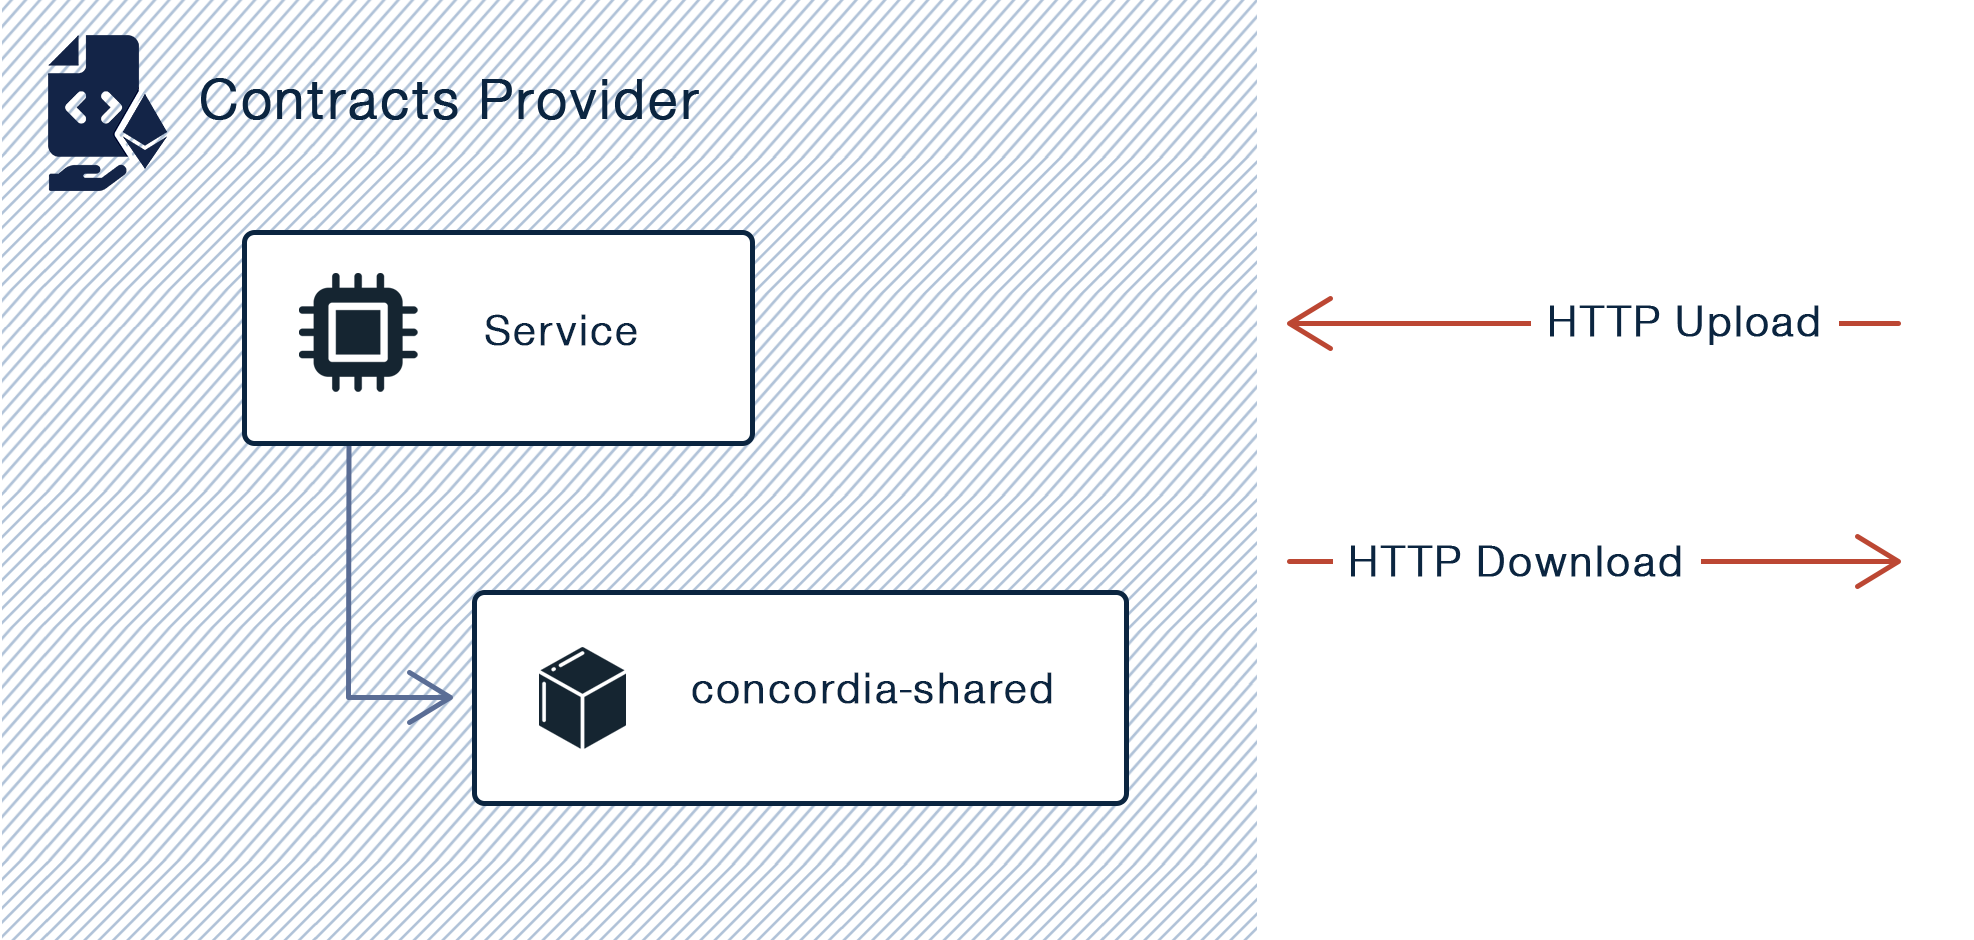
\includegraphics[width=.75\textwidth]{assets/figures/chapter-4/4.3.architecture-4.3.5.concordia-contracts-provider-architecture}
    \caption{Αρχιτεκτονική υπηρεσίας Concordia Contracts Provider}
    \label{figure:4-3-concordia-contracts-provider-architecture}
\end{figure}

Αυτή η υπηρεσία χρησιμοποιείται σε μία προσπάθεια αποσυσχέτισης της βασικής εφαρμογής που υλοποιεί η υπηρεσία Concordia Application από μία συγκεκριμένη έκδοση των contract. Οι λόγοι που αυτό είναι επιθυμητό αναπτύχθηκαν στην περιγραφή της υπηρεσίας Concordia \textenglish{Application} (υποενότητα \ref{subsection:4-3-2-concordia-application-service}). Ωστόσο, η υπηρεσία Contracts Provider αποτελεί σημείο κεντροποίησης του συστήματος και για αυτόν τον λόγο θεωρείται προσωρινή λύση για τη διευκόλυνση της προγραμματιστικής διαδικασίας. Για τη χρήση της εφαρμογής σε production, μπορεί να αντικατασταθεί με αποκεντρωτικές λύσεις, όπως με τη μεταφόρτωση και τον διαμοιρασμό των artifact μέσω του IPFS.

\subsubsection{Διανομή}

Η υπηρεσία γίνεται διαθέσιμη για χρήση ως Docker image μέσω του αποθετηρίου εικόνων Docker Hub\footnote{\url{https://hub.docker.com/r/ecentrics/concordia-contracts-provider}}. Οι χρήστες μπορούν, χρησιμοποιώντας μεταβλητές περιβάλλοντος, να αλλάξουν παραμέτρους της εκτέλεσης, όπως τη διαδρομή αποθήκευσης των μεταφορτωμένων \textenglish{contract artifact}.
\subsection{Ganache} \label{subsection:4-3-6-ganache-service}

\subsubsection{Περιγραφή - Στόχοι υπηρεσίας}

Η συγκεκριμένη υπηρεσία αξιοποιεί την CLI έκδοση του \hyperref[subsection:4-2-3-2-ganache]{Ganache}, δημιουργώντας ένα τοπικό ιδιωτικό Ethereum blockchain για τους σκοπούς ανάπτυξης της εφαρμογής Concordia.

\subsubsection{Διανομή}

Για τη χρήση αυτής της υπηρεσίας αναπτύχθηκε μία νέα εικόνα Docker που βασίζεται στην επίσημη εικόνα που διατίθεται από τη σουίτα και προσθέτει μερικές χρήσιμες λειτουργίες, όπως η δυνατότητα αποκάλυψης των κλειδιών που δημιουργούνται κατά την εκτέλεση. Η εικόνα παρέχει τη δυνατότητα τροποποίησης των παραμέτρων εκτέλεσης, μέσω της χρήσης μεταβλητών περιβάλλοντος. Με αυτόν τον τρόπο οι προγραμματιστές μπορούν να αλλάξουν τον αριθμό των λογαριασμών που θα δημιουργηθούν, το ποσό του ETH που θα λάβει κάθε λογαριασμός, καθώς και άλλες μεταβλητές.
\subsection{Rendezvous Server} \label{subsection:4-3-7-rendezvous-server-service}

\subsubsection{Περιγραφή - Στόχοι υπηρεσίας}

Η υπηρεσία Rendezvous Server παρέχει έναν signalling server, ο οποίος υιοθετεί το \hyperref[subsection:4-2-4-3-libp2p]{Libp2p} πρωτόκολλο μεταφοράς δεδομένων libp2p-webrtc-star. Μέσω αυτού παρέχεται στους ομότιμους χρήστες (peers) η δυνατότητα ανακάλυψης των διευθύνσεων των υπόλοιπων χρηστών στο δίκτυο του IPFS.

\subsubsection{Διανομή}

Αυτή η υπηρεσία είναι διαθέσιμη για χρήση από τους δημιουργούς της τόσο ως εφαρμογή μέσω του αποθετηρίου λογισμικού npm, αλλά και ως Docker image μέσω του αποθετηρίου εικόνων Docker Hub.
\subsection{Διασύνδεση υπηρεσιών} \label{subsection:4-3-8-service-communication}

Βασικό χαρακτηριστικό του μοντέλου των μικροϋπηρεσιών είναι η επικοινωνία των ξεχωριστών υπηρεσιών και η ανταλλαγή μηνυμάτων για την επίτευξη των λειτουργιών του συστήματος. Σε αυτήν την υποενότητα θα αναλυθεί ο τρόπος με τον οποίον οι μικροϋπηρεσίες επικοινωνούν μεταξύ τους, καθώς και η φύση και το περιεχόμενο των μηνυμάτων που ανταλλάσουν.

Στο παρακάτω σχήμα (σχήμα \ref{figure:4-3-communications-graph}) φαίνεται ο γράφος που οπτικοποιεί τα κανάλια επικοινωνίας μεταξύ των μικροϋπηρεσιών, καθώς και τα κανάλια επικοινωνίας των μικροϋπηρεσιών με το blockchain.

\begin{figure}[H]
    \centering
    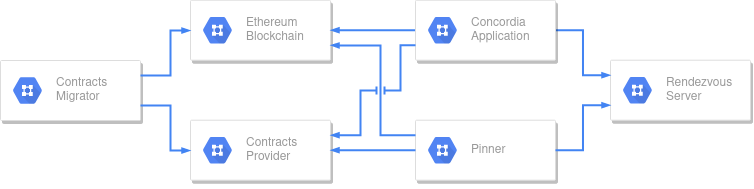
\includegraphics[width=\textwidth]{assets/figures/chapter-4/4.3.communications-diagram}
    \caption{Γράφος οπτικοποίησης των καναλιών επικοινωνίας των μικροϋπηρεσιών}
    \label{figure:4-3-communications-graph}
\end{figure}

Εδώ αναλύεται η επικοινωνία κάθε μικροϋπηρεσίας:

\begin{itemize}
    \item \textbf{Contracts Migrator}: Η υπηρεσία εκτελεί αίτημα HTTP κατά τη μεταφόρτωση των \textenglish{contract} στο Ethereum blockchain. Επίσης, εκτελεί αίτημα HTTP για τη μεταφόρτωση των \textenglish{contract artifact} στην υπηρεσία Contracts Provider.

    \item \textbf{Concordia Application}: Η υπηρεσία εκτελεί αίτημα HTTP για τη λήψη των \textenglish{contract artifact} από την υπηρεσία Contracts Provider, εκτελεί αιτήματα HTTP για τη διενέργεια συναλλαγών στο Ethereum blockchain και, τέλος, δημιουργεί κανάλι επικοινωνίας UDP με την υπηρεσία Rendezvous Server, για την ανακάλυψη ομότιμων χρηστών στο δίκτυο IPFS.

    \item \textbf{Pinner}: Η υπηρεσία εκτελεί αίτημα HTTP για τη λήψη των \textenglish{contract artifact} από την υπηρεσία Contracts Provider, εκτελεί αιτήματα HTTP για την ανανέωση και παρατήρηση της κατάστασης του contract στο Ethereum blockchain και τέλος δημιουργεί κανάλι επικοινωνίας UDP με την υπηρεσία Rendezvous Server για την ανακάλυψη peer στο δίκτυο IPFS.

    \item \textbf{Rendezvous Server}: Η υπηρεσία διατηρεί ανοιχτά κανάλια επικοινωνίας UDP με τους ομότιμους χρήστες, μέσω των οποίων ενημερώνει τη λίστα των διαθέσιμων ενεργών χρηστών.

    \item \textbf{Contracts Provider}: Η υπηρεσία δεν υποκινεί καμία επικοινωνία, παρά μόνο απαντά σε αιτήματα επικοινωνίας άλλων υπηρεσιών.
\end{itemize}
\subsection{Ροή πληροφορίας} \label{subsection:4-3-9-data-flow}

Στην παρούσα υποενότητα θα αναλυθεί η ροή της πληροφορίας στο σύστημα. Λόγω των πολλαπλών υπηρεσιών, της κατάτμησης την πληροφορίας και των διαφορετικών σημείων αποθήκευσης της, η ροή της πληροφορίας στο σύστημα ακολουθεί ένα σχετικά περίπλοκο μονοπάτι (σε σχέση με κλασσικές, μονολιθικές, κεντροποιημένες εφαρμογές).

Αρχικά θα γίνει αναφορά στη διαδικασία αποθήκευσης των νέων πληροφοριών. Η μοναδική πηγή παραγωγής δεδομένων στο σύστημα είναι οι χρήστες και κατ' επέκταση η υπηρεσία Concordia Application, εφόσον είναι η μοναδική υπηρεσία με την οποία αυτοί αλληλεπιδρούν. Τα δεδομένα που δημιουργούν οι χρήστες (πληροφορίες χρηστών, τίτλοι θεμάτων και περιεχόμενο μηνυμάτων) κατατέμνονται πριν αποθηκευτούν. Η πληροφορία που εισάγεται στο σύστημα διαχωρίζεται σε δύο μέρη. Στο blockchain αποθηκεύεται ένας δείκτης προς τα δεδομένα, ενώ τα πραγματικά δεδομένα αποθηκεύονται στη βάση OrbitDB. Ο δείκτης εκτός από την άμεση χρησιμότητα στην εύρεση των δεδομένων, παρέχει και την έμμεση λειτουργικότητα της δημιουργίας απαραίτητων μεταδομένων όπως ο αριθμός των θεμάτων στο σύστημα ή των μηνυμάτων σε ένα θέμα.

Από την πλευρά της εύρεση των πληροφοριών στο σύστημα, η ροή είναι ως εξής. Αρχικά, είναι απαραίτητη η αναζήτηση στο blockchain για την εύρεση του δείκτη προς τα δεδομένα. Έπειτα, τα δεδομένα μπορούν να ανακτηθούν μέσω του IPFS από τον εκάστοτε χρήστη ή από κάποιον Pinner.

Τέλος, παρακάτω δίνεται ένα παράδειγμα εισαγωγής πληροφορίας στο σύστημα και έπειτα ανάκτησης της ίδιας πληροφορίας.

Έστω, χρήστης που δημιουργεί νέο θέμα. Τα δεδομένα που παράγονται είναι ο τίτλος του θέματος και το περιεχόμενο του πρώτου μηνύματος. Μεταδεδομένα της δημιουργίας είναι η διεύθυνση του/της δημιουργού του θέματος. Για την αποθήκευση του θέματος στο σύστημα δημιουργείται πρώτα συναλλαγή στο blockchain ώστε να δημιουργηθεί μία νέα εγγραφή στον πίνακα των θεμάτων. Η εγγραφή αυτή δεν περιέχει τίποτα παρά μόνο τη διεύθυνση του/της δημιουργού χρήστη. Αν η συναλλαγή είναι επιτυχής, θα επιστραφεί ο αύξων αριθμός του νέου θέματος. Έπειτα, στην προσωπική βάση OrbitDB του/της χρήστη και στον πίνακα των θεμάτων θα προστεθεί εγγραφή με αναγνωριστικό τον αύξων αριθμό του θέματος όπου θα αποθηκευτούν τα δεδομένα του τίτλου και πρώτου μηνύματος. Στο σχήμα \ref{figure:4-3-data-flow-insert} παρουσιάζεται γραφικά η διαδικασία.

% todo: UML diagrams might be wrong, should the ethereum and orbitDb blocks be continuous?
\begin{figure}[H]
    \centering
    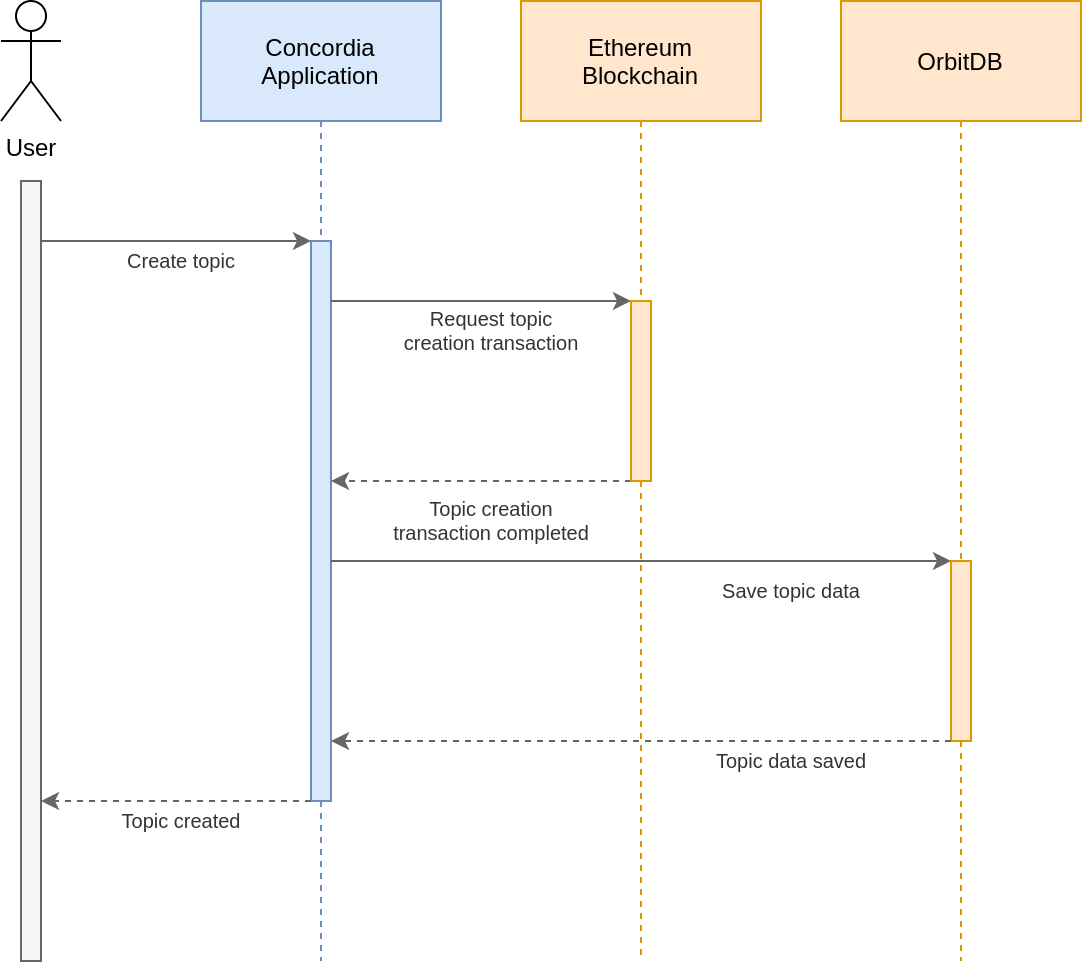
\includegraphics[width=.7\textwidth]{assets/figures/chapter-4/4.3.architecture-4.3.9.data-flow-insert.png}
    \caption{Διάγραμμα ακολουθίας δημιουργίας θέματος}
    \label{figure:4-3-data-flow-insert}
\end{figure}

Έστω, χρήστης που επιθυμεί να διαβάσει το προηγούμενο μήνυμα. Αρχικά, πρέπει να διαβαστεί ο πίνακας θεμάτων από το blockchain. Η πληροφορία αυτή εμπλουτίζεται από τα δεδομένα του κάθε θέματος, τα οποία ανακτώνται από τις προσωπικές βάσεις Orbit κάθε χρήστη. Έπειτα, εφόσον το θέμα βρεθεί και ο αύξων αριθμός του είναι γνωστός, πρέπει να διαβαστούν από το blockchain τα μεταδομένα των μηνυμάτων του θέματος και συγκεκριμένα η διευθύνσεις των δημιουργών τους. Τέλος, μέσω του IPFS πρέπει να γίνει αντιγραφή των προσωπικών βάσεων των δημιουργών του κάθε μηνύματος και να αναζητηθούν σε αυτές τα εκάστοτε μηνύματα. Στο σχήμα \ref{figure:4-3-data-flow-read} φαίνεται το διάγραμμα ροής της πληροφορίας κατά την ανάκτηση πληροφοριών από το σύστημα.

\begin{figure}[H]
    \centering
    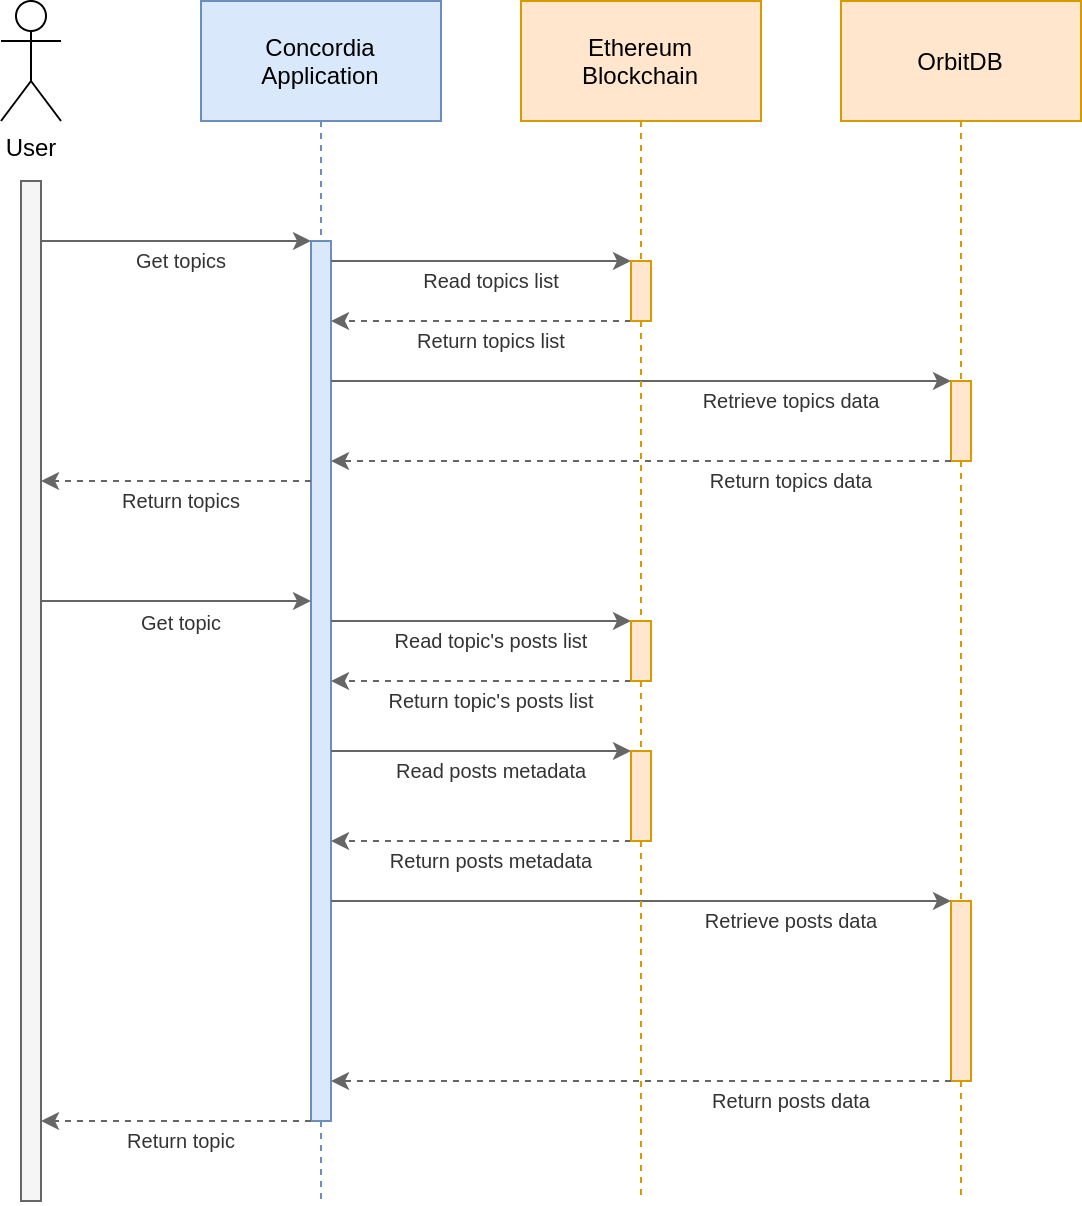
\includegraphics[width=.7\textwidth]{assets/figures/chapter-4/4.3.architecture-4.3.9.data-flow-read.png}
    \caption{Διάγραμμα ακολουθίας εύρεσης και ανάκτησης θέματος}
    \label{figure:4-3-data-flow-read}
\end{figure}